% !TEX encoding = UTF-8 Unicode

\documentclass[9pt]{amsbook}
\usepackage[b5paper,margin=1in]{geometry}
\usepackage{kerbal-book}
\usepackage{graphicx}

\usepackage{tikz}
\usepackage{pgfplots}
\usepackage{mathtools}

\usepackage{multirow}
%\usepackage[korean]{babel}


\usepackage{makecell}

\usepackage{threeparttable}
\usepackage{standalone}
\usepackage{booktabs, dcolumn}

\usepackage{subfig}
\usepackage{footnote}
\makesavenoteenv{tabular}
\makesavenoteenv{table}

%\setlength{\voffset}{- 0.3 in}
\setlength{\footskip}{40pt}

\setlength{\parindent}{1.2em}
\setlength{\parskip}{0.8em}
\renewcommand{\baselinestretch}{1.5}

\newcommand{\dia}{$\diamondsuit$}

\newcommand{\ttuna}{\textsuperscript{$\dagger$}} % Table Note 1
\newcommand{\ttsecu}{\textsuperscript{$\ddagger$}} % Table Note 2


\usepackage{fancyhdr}
\usepackage{pdflscape}
\usepackage{longtable}

\title{kerbal-book}
\author{Alberto Liberio Humaniense Disciplino}
\date{March 2016}

\begin{document}

\maketitle
\sf
%\frontmatter
\chapter*{Kerbal Space Program이란?}
Kerbal Space Program (약칭 KSP) 란 Squad사에서 만든 우주선 시뮬레이션 게임입니다.
뉴턴역학, 로켓역학

이 게임은 그저 실제에 충실히 뉴턴역학을 구현하는 데에만 신경을 쓴 것은 아닙니다. 실제 태양계보다 축소된 모델로 우주선을 궤도에 올리는 것을 실제보다 용이하게 해놓은 것이 많은 사용자들이 더 쉽게 플레이 해볼 수 있게 하는 장점을 가지고 있습니다. 게임에 등장하는 우주비행사도 인간이 아닌 작고 귀여운 녹색인간으로, 캐릭터성 또한 겸비하고 있습니다.

딸도 달미션 했다 리뷰 소개

여러가지 물리현상 (스킬) 소개

교육에도 활용할수 있고 적극 추천중. 플레이 영상 업로드도 공식 허가.

ksp는 왜 좋은가
-교육

하지만, 새롭게 이 게임을 시작하는 사람들이 진행에 많은 어려움을 겪는 것을 보았습니다. 이 서적의 목적은 크게 두 가지입니다. 
우선, 처음 입문하는 사람들이 쉽게 따라하면서 게임을 이해할 수 있는 입문서로서의 목적이 있습니다.
또한, 가능한한 많은 수치표를 넣어 숙련자들도 이용할 수 있는 계산툴로서 기능하게 하는 목적이 있습니다.
최대한 첫째 목적을 이루는 것이 주 목표이며, 이를 지키면서도 최대한 많은 물리현상들을 설명하고, 또 정교한 스킬들을 익힐수 있게 하고자 합니다.
짧은 집필기간과 계속되는 게임의 업데이트 때문에 초판은 충분히 잘 기술되지 못할 수 있을 것입니다.
게임소스를 제외한 본 서적의 핵심적인 부분인 기술적인 설명과 저자의 개인연구 부분은 오픈소스 라이센스 하에 있으며, 앞으로 독자들께서도 자유롭게 편집할 수 있도록 할 것이오니,
혹시 틀린 점을 발견하거나 추가하고 싶은 내용이 있으면 책 마지막 장의 소스 URL에서 추가해주시길 부탁드립니다.


\tableofcontents
%\mainmatter
\part{시작하기}
\chapter{궤도에 올리기}
\section{운동에너지 얻기}
\paragraph{일의 공식}
일의 공식은 $W=\vec{F} \cdot \vec{v} = F v \cos\theta$이다. 
즉, 힘의 방향이 운동방향과 나란할 수록 얻는 운동에너지가 많아진다. 
따라서 로켓을 발사할 때는 속도 방향과 최대한 가까운 방향으로 가속해주는것이 가속효율에 도움이 된다.
단, 에너지는 기준계에 따라 달라지므로 어떤 기준계에서 생각하는지가 중요하다. 
어떤 행성 주위에 궤도를 형성하고 싶다면 그 행성을 기준으로 한 좌표계에서 생각해야 한다. 
KSP에서는 어떤 행성이나 위성 가까이에 있으면 그 별을 중심으로 하는 관성계를 기준으로 삼고 있다 (comoving inertial frame). 
태양이나 모행성에 의한 기조력은 생각하지 않고 있으므로 훨씬 간단하게 계산할 수 있지만, 또한 나름 실제와 비슷한 현상을 이와 같은 저차근사에서도 볼 수 있다. 
주의해야 할 점은 기준계를 행성표면을 따라 자전하는 좌표계로 잡게 되면 비관성계의 역학을 적용해야 하므로 뉴턴역학을 적용할 수 없다는 점이다. 
따라서, 공기역학을 다루지 않고 순전히 탄도학만 생각할 때는 관성계를 항상 기준으로 해야함을 잊지 않아야 한다.

단, 대기밀도가 높은 곳에서는\footnote{고도 40km이하, 정확한 데이터가 있으면 추가바람.} 지표면에 대한 좌표계를 써야한다. 즉, 대기와의 상대속도를 기준으로 잡아야한다. 공기역학적 힘이 로켓의 궤도와 안정성에 큰 영향을 미치므로, 대기에 대해 빠른 속도를 얻어 대기를 빨리 탈출하는 것이 에너지 손실을 막는데도 도움이 되기 때문이다.

\paragraph{Gravity turn}
처음 로켓을 발사할 때는 수직으로 발사하게 된다. 하지만 행성 주변으로 원운동 (혹은 타원운동)을 하게 하기 위해서는 지면과 수평방향의 속도를 주는 것이 중요하다. 
이 때, 로켓의 방향을 수직에서 수평으로 눕혀주는 속도가, 앞에서 말한 바와 같이 에너지 효율에도 중요하고, 로켓의 공기역학적 안정성에도 중요하다. 
이러한 각도변화는 인위적으로 조정해야 하지만 (pitch manuever) 어느 정도 중력에 의해 자연적으로 일어난다 (gravity turn).
여기서는 이러한 turn이 자동적으로 이루어지는 이유와 정도에 대해서 우선 설명하고, 그 다음 이러한 turn을 얼마나 조정해야 하는지 설명하도록 할 것이다.

우선, 처음 로켓을 발사하게 되면 바로 동쪽으로 살짝 머리를 돌려야 한다. (5도 정도) 그 이유로는 
\begin{itemize}
\item 수직으로 발사했을 경우, 로켓이 추락하면 발사대가 파괴된다.
\item 여기서 기술할 gravity turn을 만들기 위해서이다.
\item 로켓이 진행방향을 바꾸지 않고 그대로 진행할 경우 코리올리 힘에 의해 머리는 점점 서쪽으로 기울게 된다. (우리가 가고자하는 방향과 반대방향.)
\end{itemize}
참고로 여기서는 동쪽방향으로 궤도를 만드는 것을 가정하고 있다. Kerbin의 자전속도를 이용할수 있어 더 효율적으로 쏘아올릴 수 있기 때문이다.
한번 어느정도 머리가 동쪽으로 기울게 되면, 중력가속도에 의해 로켓의 속도는 수직방향의 가속도를 계속 받게 되므로 아래방향으로 계속 기울게 된다. (참고: Figure \ref{fig:gravturn})
따라서, 이러한 gravity turn은 pitch manuever에서 도움도 주지만, 반대로 초기의 기울임 값을 너무 크게 주게 되면 기울어지려는 경향이 너무 커져서, 대기권을 탈출하기에는 너무 낮은 궤도가 형성될수 있으므로 주의해야 한다.

\begin{figure}
\caption{Gravity turn. 중력가속도에 의해 로켓의 속도는 점점 아래로 처지게 된다.}
\label{fig:gravturn}
\includegraphics[width = 0.3\textwidth]{gravityturn.png}
\end{figure}

이런 자연적인 turn에 의존하여 발사를 성공할 수 있다면, 로켓의 추력은 계속 속도방향과 평행하므로 에너지 효율면에서 최대의 효과를 얻을 수 있다. 하지만, 이러한 초기값 찾기 문제는 상당히 어렵고, 오차가 발생하더라도 궤도 보정을 할 수 있어야 하므로, 머리방향을 원하는 대로 움직이는 pitch manuever를 하게 된다. 
나중에 공기역학에서 다루겠지만, 공기에 대한 상대속도에서 큰 각을 주는 방향으로 머리를 움직이는것은 에너지 효율뿐 아니라 로켓의 안정성을 해치므로 해서는 안되는 일이지만,
로켓이 공기저항을 적게 받는 층으로 들어가려고 할때나, gravity turn이 너무 많이 이루어져서 궤도를 높게 수정할 필요가 있을때, 로켓이 머리를 돌려야 하는 경우가 발생할 수 있다.

다음번 인쇄시에는 여기에 각각의 경우에 해당하는 정확한 수치등을 기록하려 한다.



\section{공기역학 및 안정성}
로켓을 쏘아올리는 단계에서 탄도학으로 알 수 없는, 가장 중요한 요소가 바로 공기저항이다. 
운동방정식은 무게중심에서 써지지만, 공기역학적인 힘은 물체의 부피중심에 작용한다. 
로켓에 작용하는 힘을 생각해보자: 중력은 무게중심에 작용하고, 공기역학적인 힘은 부피중심, 그리고 엔진의 추력은 로켓의 밑부분에서 발생한다. 그런데, 보통 로켓은 아랫단으로 갈수록 윗단을 나르기 위해 더 힘이 세고 무거운 로켓으로 구성되어 있다. 따라서, 무게중심은 부피중심보다 아랫쪽에 있는 경우가 많다. 무게중심보다 윗쪽 작용점에서 공기저항력이 아랫쪽으로 작용하고, 추력이 아랫쪽에서 윗쪽을 향해 작용하므로, 로켓은 근본적으로 불안정하게 된다.

이는 엔진이 로켓의 가장 밑부분에 있어서 발생하는 문제로, 설령 부피중심이 아랫쪽에 있다고 해도 (덜하긴 하지만) 똑같이 돌림힘이 생기므로 로켓은 거꾸로 뒤집어지려고 한다.

해결방법을 여러가지 생각해볼 수 있을것이다.
\begin{itemize}
\item 엔진을 무게중심보다 위에 단다.
\item 공기저항을 많이 받는 물건을 아랫쪽에 붙여서 조금더 안정성을 높인다.
\item 돌림힘을 발생하는 장치를 마련한다.
\end{itemize}

첫번째 해결법에서는 엔진을 연료통 옆에 붙일 수 밖에 없으므로 면적이 늘어나고 공기저항도 증가하여 효율적이지 못하다. 또한, 공기저항의 작용점을 오히려 위쪽으로 이동시켜서 불안정해질수 있는 요소도 있다.
세번째 해결법은 대부분 Command Module에 탑재되어 있다. 거대한 자이로스코프를 이용하여 자세제어를 하지 않으면, 로켓은 근본적으로 불안정하므로, 이러한 장치가 기본적으로 장착되어 있으나, 로켓의 규모에 비해 만들수 있는 힘이 작고, 전기도 소비하므로 이 또한 효율적이지 않다.
두번째 해결법이 세번째 해결법을 보완하기 위해 나온것이다. 로켓 아랫쪽에 날개를 붙이게 되면 공기역학적 작용점이 아래로 내려가서 자이로스코프만으로도 자세제어가 가능해지고, 또한 이 날개가 움직이기까지 한다면 공기역학적인 힘을 이용하여 자세제어도 가능하게 되는것이다.

\begin{figure}
\caption{로켓의 추력과 공기저항은 로켓이 공기역학적으로 불안정하게 한다. }
\begin{center}
\includegraphics[width=0.5\textwidth]{aero.png}
\end{center}
\end{figure}

로켓을 만들 때 있어서 주의해야 할 점은,
\begin{itemize}
\item 날개를 붙인다;
\item 로켓을 너무 길게 하지 않는다;
\\
로켓을 너무 길게 하게 되면, 작용점사이의 거리가 멀어져서 (필요한 돌림힘이 커지므로) 불안정하게 되고,
또한 로켓자체의 내구성이 이러한 큰힘을 이기지 못하고 부러져버릴 수도 있다.
\item 그리고 로켓이 '지표면좌표계에서의' 속도방향과 머리의 방향이 5도 이상 차이나지 않게 한다.
\\
이미 90도 꺾여버린 로켓을 상상해보자. 더이상 컨트롤할 수 없게 된다. 공기에 대한 속도와 머리방향의 차이를 크지 않게 하여 불안정한 힘이 커지지 않게 하는것이 중요하다.
\end{itemize}

로켓역학에 있어서 대기층은 크게 세가지로 나눌수 있을 것이다.
\begin{itemize}
\item 대류권(0$\sim$20km, 성층권 상층부 포함): 공기가 너무 밀하여, 엄청난 공기저항을 받는 층. 발사시에도, 재진입시에도, 로켓은 보통 비행기 이상의 속도를 낼수 없으며(마하 2$\sim$3), 재진입시 낙하산이 펴지는 곳도 이곳이다.
\item 성층권, 중간권 (20$\sim$50km): 보통 재진입시 최저지점을 여기로 잡는다. 비행기는 날수 없지만 빠른 속도에서는 충분한 공기저항을 만들어서 감속하여 대류권으로 진입하게 해준다. 로켓발사시에는 주로 가속을 하는 구간이 여기이며, 아직 공기저항이 충분히 남아있으므로 방향전환에 주의해야한다.
\item 열권 (그 이상): 행성탐사등 아주 먼거리를 다녀와서 초고속으로 통과할때는 불꽃이 생길 정도이지만, 제대로 된 감속을 해주지는 못한다. 발사시에는 안심하고 머리를 틀 수 있는 곳이다.
\end{itemize}
대류권 상층부에 보통 MaxQ 지점이 존재한다. MaxQ란 로켓발사중에 공기역학적 힘을 최대로 받는 지점을 얘기하며, 상승할 수록 속도는 증가하나 공기밀도가 감소하므로 이처럼 중간 지점에 존재하게 된다. 게임을 초반에 진행할때 MaxQ 이전에 보통 공기역학적 문제점들이 드러나며, 이를 통과하면 문제가 발생할 확률이 줄어든다.

\paragraph{Over-compensating}
로켓이 기울려고 하면 reaction wheel을 이용하여 로켓을 반대편으로 기울도록 하는 힘을 주어야 한다. 
이런 compensating한 기동은 안정화가 필요한 모든 시스템에서 필요하다. 
예를 들자면 자동차도 한 쪽으로 미끌어지려고 할 때 반대쪽으로 카운터스티어링을 해주어야 하는 것처럼 말이다. 
로켓에서는 이를 자동으로 해주는 컴퓨터 시스템이 존재하는데 이를 SAS\footnote{키브드에서 'T'키를 누르면 활성화/비활성화 된다.}라고 한다. 
이 시스템은 로켓이 오른쪽으로 기울면 왼쪽으로, 왼쪽으로 기울면 오른쪽으로 힘을 준다.

문제는 이 시스템이
\begin{itemize}
\item 필요한 것에 비해 주어지는 돌림힘이 너무 크고
\item 반응이 즉각적이다.
\end{itemize}
마치 운전 비숙련자가 카운터 스티어링을 타이밍 안졸게 과도하게 해서 오히려 차를 불안정하게 하거나, 그네를 타이밍좋게 밀면 왕복운동이 점점 커지는것처럼, 로켓은 바른 방향에서 점점 멀리까지 운동하고 불안정성을 증가시키게 된다.

이 경우는 과도하게 compensating되는 경우이므로, SAS를 끄고, 침착하게 천천히 목표하는 방향을 향해 조작을 하는것이 안정성을 회복하는데에 도움이 된다. 

무엇보다, 
\begin{itemize}
\item 로켓의 질량에 비해 충분한 돌림힘을 낼 수 있게 설계하고
\item 주어지는 힘에 비해 로켓의 내구성이 충분하도록 로켓을 길게 하지 않고 구조를 보강하면
\end{itemize}
이런 상황은 방지할 수 있다.

\section{재진입시 주의사항: 방열판 (Heat Shield)}
우주선의 대기속을 빠른 속도로 지나가게 되면, 우주선 앞쪽에는 다른 곳으로 가지 못하고 우주선 앞부분에 공기입자들이 쌓이게 되고, 반대로 우주선 뒷부분은 주변보다 공기가 적게 된다. 또한, 이런 과정은 순식간에 일어나므로, 단열압축, 단열팽창에 해당된다. 따라서, 우주선 앞부분의 고기압은 '공기저항'을 만들어 우주선을 감속시켜 주기도 하지만, 단열압축으로 인한 막대한 열로 우주선을 위협하기도 한다.

특히, 고고도에서 수직낙하할 경우에는, 
일반적인 우주여행에서 있을 수 없는 정도의 극한적인 공기저항을 받게 되므로 우주선이 타버리게 된다. 
처음 KSP를 시작하고 로켓제작에 아직 적응되지 않았을 때, 
로켓이 내는 에너지가 충분한지 알기 위해 수직발사 하는 경우가 
있을 수 있는데,\footnote{공기저항을 무시하면 대략 고도 740km이상 올라갈 수 있으면 저궤도를 구성할 수 있다.}
일반적인 경우처럼 수평과 가깝게 대기권에 들어오지 않고 거의 수직으로 대기에 재진입하게 되므로,
충분히 감속되기 전에 밀도가 높은 대기를 만나게 되어 아주 높은 열을 
내게 된다.\footnote{사실 가장 낮은 궤도에서 재진입하는 경우 v1.03에서는 방열판 없이도 살아남을 수 있지만, 
이것이 거의 유일한 상황이다.} 
따라서, 처음 로켓을 만드는 분들도 Command module밑에 방열판을 붙이는 것을 잊지 말아야 한다.

\paragraph{단열압축}
일반적인 공기저항 공식은 다음과 같다.
\begin{align}
\Delta P = \frac{C}{2} \rho v^2 = \frac{C}{2} v^2\frac{m P}{kT}
\end{align}
여기서 $m$은 공기의 평균 분자 하나당 질량이다.

여기서 이원자분자기체의 단열압축 공식은 $P^{-2}T^7=const$이므로, $\Delta P$를 $\int dP$로 해석해서 연속체공식을 구하면 다음과 같다.
\begin{align}
	\frac{7}{2}\Delta(P^{2/7}) = \frac{mP_0^{2/7}}{kT_0} \frac{Cv^2}{2}
\end{align}
제대로된 우주선의 재진입이라면 대기의 상층부에서 대부분의 감속이 일어나므로, 저압력점이 고압력점에 비해 배경 압력과 차이가 많이 나지 않는다고 가정하면, 물체 앞쪽의 단열압축에 의한 온도상승은 다음과 같다.
\begin{align}
T-T_0 = \frac{mCv^2}{7k}
\end{align}
KSP에서는 재진입 상황에서 2700K(2300m/s)에서 14000K(53000m/s)까지 도달할 수 있다. 우주선의 내열 온도는 보통 1000도 정도이므로 반드시 방열판을 설치해야만 우주선을 보호할수 있다.

\paragraph{카탈로그}
\par
\begin{threeparttable}
\caption{방열만의 종류}
\begin{tabular}{|r|r|r|r|r|}
\hline
크기&질량& Max. Temperature& 내구 충돌속도& Ablator
\\\hline
1.25\,m&0.3\,t& 3300\,K&9\,m/s&200
\\2.50\,m&1.3\,t&3300\,K&9\,m/s&800
\\3.75\,m&2.8\,t&3300\,K&9\,m/s&1800
\\10.00\,m&1.5\,t&3500\,K&9\,m/s&-
\\\hline
\end{tabular}
\end{threeparttable}

여기서 Max. Temperature의 의미를 혼동해서는 안된다. 저자의 추측이지만 (검증바람) Max. Temp.에 도달하고 나서 부품이 바로 부서지는 것이 아니라, 그 온도 이상부터는 부품의 내구도를 소비하게 되고, 내구도가 떨어지면 파괴된다. (그렇지 않다면 내구도가 닳기 시작하는 온도가 따로 써져 있어야 할텐데 그런 온도는 없다.) 따라서, 방열판도 Max. Temp.가 되서부터야 Ablator를 소비할 것이다.

Ablator란 방열판의 양으로서, 방열판은 고온에서 기화되면서 열을 흡수하게 된다. Max. Temp. 이상이 되면 방열판의 Ablator가 소비되기 시작하고, 이것이 떨어지면 방열판은 더 이상 기능할 수 없게 된다.
\paragraph{매뉴버}
Command module에는 방열판에 거의 수직하는 공기저항이 작용한다. 실제 아폴로 미션에서는 Command module의 무게중심을 중심축에서 비껴가게 하여, 방열판이 정면을 보지 않고 약간 기울어 진 자세가 가장 안정한 자세가 되게 하였다. 그렇게 하면 우주선이 기울어진 방향으로 공기역학적인 힘이 작용하여 착륙지점을 이동시킬수 있다. 다른 방향으로 움직일때는, 속도방향축을 중심으로 Roll을 하였다.

우주선이 다른방향으로 회전(Pitch, Yaw) 하는 것은 거의 불가능하다. 안정한 자세가 아니기 때문에 자세를 유지하기 위해 막대한 에너지를 소비하기 때문이다. 배터리를 충분히 준비한다면 가능하긴 하다. 사실, KSP에서는 무게중심을 이동시켜서 비대칭으로 만드는것보다는 이렇게 전기를 이용하여 Pitch나 Yaw를 하는데 더 나을수 있다. 왜냐하면 무게중심을 이동시키기 위해서는 질량이 있는 물체를 Command module에 매달수 밖에 없는데, 물체자체의 부피 때문에 무게중심의 이동만큼 공기저항의 작용점이 이동하기 때문이다. KSP에서는 이렇게 공기역학을 이용한 재진입시 매뉴버는 힘들다고 볼 수 있겠다.

\begin{figure}
\caption{Command Module이 대기에 비스듬히 진입할때 생기는 힘}
\includegraphics[width=0.3\textwidth]{lift.png}
\end{figure}

\section{재진입시 주의사항: 낙하산 (Parashute)}
재진입 마지막 단계에서 수평방향의 높은 속도를 잃어버린 우주선은 거의 수직으로 낙하하게 된다. (고도 11\,000\,m $\sim$ 7\,000\,m) 이 단계에서는 우주선이 대기와의 마찰로 불꽃을 일으킬 정도는 아니지만 여전히 낙하산을 펴기에는 높은 속도일 수 있다. 자유낙하하면서 충분히 저속이 될 때까지 기다린 후 낙하산을 작동시켜야 한다. 그렇지 않으면 낙하산은 파괴되고 우주선은 지상에 충돌하여 소멸하게 될 것이다.

우주선을 설계할 때는 마지막에 착륙하게 될 우주선이 이러한 자유낙하를 통한 감속 후에도 낙하산을 펼 수 있는 충분한 고도를 확보할 수 있는지 검토해야 한다. Kerbin에 고속으로 재진입후에는 각도에 따라 낙하산을 펼 수 있을만큼 감속하는 고도가 7\,000$\sim$5\,000\,m가 되기도 하는데, 산악지형이라면 지면에 충돌할 수 있다. 따라서 산악지형에 착륙하지 않도록 피하는 것도 중요하다.

마지막으로, 낙하산의 의미는, 낙하산이 완전히 펴졌을 때의 속도가 우주선이 견딜만한 충돌속도가 되게 하는 것이므로, 낙하산의 면적에 비하여 우주선이 너무 무겁지 않은지 검토해야 한다. 저고도발사후 Command Module을 분리하여 낙하산을 펴보는 것으로 종단속도를 간단히 확인할 수 있다.

낙하산의 종류는 Table \ref{table:parachute}와 같다. 낙하산의 종류는 두가지가 있는데, 일반적으로 재진입 마지막 단계에서 속도를 줄이기 위한 Parachute와 초음속에서 속도를 줄이기 위한 Drogue Chute가 있다. 대기가 희박한 행성에서는 Parachute가 펴질정도로 충분한 감속이 이루어지지 않은 상태에서 지표에 접근하게 되므로 Drogue Chute가 필요할 수 있다.

\begin{center}
\begin{adjustbox}{width=\textwidth}
\begin{threeparttable}
\caption{
낙하산의 종류
(From Wiki and Game). 
낙하산은 작동되면 반쯤 펴진상태가 되며 설정된 고도에서 전부 펴진다. 
낙하산이 만들어내는 공기저항은 $F = 1/2 \,\rho A v^2$이다. 
여기서 $\rho$는 공기의 밀도, $A$는 아래 표의 반지름에서 구할수 있는 낙하산의 면적이다.}
\label{table:parachute}
\begin{tabular}{|l|l|r|r|r|r|r|}
\hline
용도&이름&크기&작동최대속도&작동최저기압&접힌반지름$^\dagger$&펴진반지름$^\ddagger$
\\\hline
\multirow{3}{*}{Parachute}&Mk16&0.625\,m&\multirow{3}{*}{264\,m/s}&\multirow{3}{*}{0.04\,atm}
&0.4\,m&20.7\,m
\\
&Mk16-XL&1.250\,m&&&1.3\,m&37.8\,m
\\
&Mk2-R &Radial-Mount&&&0.8\,m&30.4\,m
\\\hline
\multirow{2}{*}{Drogue Chute}&Mk25&1.250\,m&550\,m/s&\multirow{2}{*}{0.02\,atm}&0.7\,m&4.7\,m
\\
&Mk12-R &Radial-Mount&424\,m/s&&0.7\,m&5.6\,m
\\\hline
\end{tabular}
\begin{tablenotes}
\item[$\dagger$] semi-deployed
\item[$\ddagger$] fully deployed
\end{tablenotes}
\end{threeparttable}
\end{adjustbox}
\end{center}


\paragraph{legacy: v1.0 미만에서의 자유낙하}
가장 일반적으로 쓰이는 공기저항 공식은 면적에 비례하지만, 
베타버전에서는 물리모델을 더 단순화시키기 위해 공기저항은 물체의 질량과 공기저항계수의 곱에 비례했다.
대부분의 물체의 저항계수는 1이었으므로,
대부분의 물체에 적용되는 종단속도가 존재했다.
또한, 대기모델도 압력이 지수함수로 감소하는 단순한 모델을 가지고 있었으므로,
공기저항에 의한 궤도변화도 계산하기 쉬웠다.

당시 공기저항 모델과 저자가 측정한 공기저항계수는 (아마 exact) 다음과 같았다.
\begin{align}
F_{drag}&=-(9.784\times 10^{-4}\, \mathrm{atm}^{-1}\mathrm{m}^{-1})\, p\, v^2
\\p&=(1 atm)\,e^{-h/h_0}
\\1\,\mathrm{atm} &:= 101325\,\mathrm{Pa}
\\h_0&:= 5\,600\,\mathrm{m}
\end{align}
이 때의 고도에 따른 종단속도(마찰계수 1)은 Table \ref{table:obslete}과 같다.
\begin{table}
\begin{center}
\begin{threeparttable}
	\caption{베타 버전에서의 고도에 따른 종단속도. 이 때는 global한 종단속도가 존재했다.
	 (From Wiki and 직접계산)}\label{table:obslete}
		\begin{tabular}{|r|r|r|r|r|}
			\cline{1-2}\cline{4-5}
			height& term. speed&&height& term. speed
			\\\cline{1-2}\cline{4-5}
			1\,000\,m&110.5\,m/s$^\flat$ && 20\,000\,m&716.0\,m/s
			\\\cline{1-2}\cline{4-5}
			2\,000\,m&121.9\,m/s && 23\,000\,{m}&961.9\,m/s
			\\\cline{1-2}\cline{4-5}
			3\,000\,m&134.5\,m/s && 25\,000\,{m}&1171.1\,m/s
			\\\cline{1-2}\cline{4-5}
			4\,000\,m&148.4\,m/s && 30\,000\,{m}&1915.4\,m/s
			\\\cline{1-2}\cline{4-5}
			5\,000\,m&163.7\,m/s && 32\,000\,{m}&2332.1\,m/s
			\\\cline{1-2}\cline{4-5}
			6\,000\,{m}&180.6\,m/s && 32\,136\,{m}&Max enter periapsis\ttuna
			\\\cline{1-2}\cline{4-5}
			7\,000\,{m}&199.3\,m/s && 35\,000\,{m}&3133.2\,m/s
			\\\cline{1-2}\cline{4-5}
			8\,000\,{m}&219.9\,m/s && 40\,000\,{m}&5125.4\,m/s
			\\\cline{1-2}\cline{4-5}
			9\,000\,{m}&242.6\,m/s && 45\,000\,{m}&8384.8\,m/s
			\\\cline{1-2}\cline{4-5}
			10\,000\,{m}&267.7\,m/s && 50\,000\,{m}&13717.9\,m/s
			\\\cline{1-2}\cline{4-5}
			12\,500\,{m}&342.4\,m/s && 55\,000\,{m}&22444.3\,m/s
			\\\cline{1-2}\cline{4-5}
			15\,000\,{m}&437.8\,m/s && 60\,000\,{m}&36724.0\,m/s
			\\\cline{1-2}\cline{4-5}
			\multicolumn{3}{r|}{}&69\,077\,{m}&End of atmosphere\ttsecu
			\\\cline{4-5}
		\end{tabular}
	\begin{tablenotes}
		\item [$\dagger$] \small 물체가 멀리서부터 대기로 진입할 때 이 고도보다 낮은 고도가 근지점인 궤도로 들어오면
						 공기저항이 충분하여 Kerbin에 무사히 착륙할 수 있다.
						 현재 버전에서는 이 고도보다 낮아진 듯 하다. (우주선 모양에 따라 다름)
		\item[$\ddagger$] $10^{-6}\,\mathrm{atm}$이 되는 고도이다. 여기서부터는 대기가 없는 것으로 가정하고 공기역학은 계산되지 않는다. 정식 버전의 대기모델은 훨씬 복잡하고 (지구처럼 층 구조가 있다) 대기가 끝나는 것으로 가정하는 고도는 70\,000\,m\,로 딱 떨어지는 숫자로 맞추어 놓았다. 다른 행성의 경우에는 지표면 기압의 $10^{-6}$가 대기 한계였다. 
		\item[$\flat$] 지표면 가까운 곳에서의 (10km 이하) 종단속도는 Command Module의 경우 (보통 Kerbin 귀환시) 이 속도보다는 정식버전에서 낮아져있다.
	\end{tablenotes}
\end{threeparttable}
\end{center}
\end{table}

\chapter{다단 로켓과 $\Delta v$}
\section{연료}

\begin{align}
    \Delta v =I_{sp}\, g_0\log\frac{M+m}{M}
\end{align}

\begin{align}
    \Delta v = I_{sp}\, g_0\log\frac{M+(1+\alpha) m}{M+\alpha m}
\end{align}
\begin{align}
    \Delta v \rightarrow I_{sp}\, g_0\log(1+\alpha^{-1})
\end{align}

is independent of thrust force but only depend on isp and etc

Let's assume $I_{sp} =320 s$ and 

Estimated Engine Mass / Fuel Mass = 1/6

Estimated Fuel Tank Mass / Fuel Mass = 1/8

$\Delta v = 4669.78 m/s$

실제로는 1단의 경우 공기저항으로 인해 연료를 많이 실을 수록 오히려 얻을 수 있는 운동에너지가 줄어드는 결과를 보이기도 한다. 따라서 많은 양의 화물(Load)을 쏘아 올리기 위해서는 `다단 로켓 (multi-stage rocket)'과 `아스파라거스 로켓 (asparagus-staging rocket)'이 필요하다.


%{\fontfamily{omyglm}가나다}
%{\fontfamily{omyglm}\selectfont가나다}
%{\fontfamily{unbtbco04}\selectfont가나다}
\section{다단 로켓 (Linear Staging)}
a


\section{아스파라거스 (Asparagus Staging)}

\section{$I_{sp}$}
\begin{align}
I_{sp} = \frac{F}{\dot{m}g_0}
\end{align}


\chapter{궤도운동}
\section{용어설명 및 주의사항}
*근일점은 꼭 태양과 지구사이만의 의미가 아니고 일반적으로 사용할것임
\section{원궤도}
\section{타원궤도}
별 (start) 우주선 (projectile) 위치에너지 (potential energy)
\begin{align}
&r^2 \dot{\theta} = l
\\&\ddot{r}-\frac{l^2}{r^3}+\frac{GM}{r^2} = 0
\end{align}
\begin{align}
	-l^2r^{-2}\frac{d^2r^{-1}}{d\theta^2}-l^2r^{-3}+GMr^{-2} = 0
\end{align}
\begin{align}
	\frac{d^2r^{-1}}{d\theta^2}+r^{-1}-GMl^{-2} = 0
\end{align}

이러한 우주선(projectile)의 운동방정식의 해는 다음과 같다.
\begin{align}
	r^{-1} = \frac{GM}{l^2} + \sqrt{\frac{2\epsilon}{l^2}+\left(\frac{GM}{l^2}\right)^2}\cos(\theta+\theta_0)
\end{align}
여기서 $\epsilon$은 우주선(projectile)의 질량당 총 에너지이다. 이러한 식은 이차곡선(원, 타원, 포물선, 쌍곡선)을 나타내는 표현이다. 따라서 이는 역제곱힘에서의 궤도가 이차곡선이 된다는 증명이다.
이 식을 $l$과 $\epsilon$이 아닌 $l$과 근일점($r_p$)의 함수로 나타내면 다음과 같이 나타낼 수도 있다.
\begin{align}
	r^{-1} = \frac{r_p^{-1}}{2}\cdot\frac{1}{1+\epsilon (GM)^{-1}r_p} +\frac{r_p^{-1}}{2}\cdot\frac{1+2\epsilon (GM)^{-1}r_p}{1+\epsilon (GM)^{-1}r_p}\cos(\theta+\theta_0)
\end{align}
$r$이 무한대로 가지 않고 유한한 영역에서 진동하고 있으면 원이나 타원, 즉 구속궤도(bound orbit)이 되고, $r$이 무한대, 즉 $r^{-1}=0$인 지점이 있으면 비구속궤도(unbounded orbit)가 될 것이다.

\section{쌍곡선궤도 - 탄성충돌}
\section{슬링샷}

\begin{align}
	\Delta \theta = \pi + 2\sin^{-1}\frac{1}{{1+2\epsilon (GM)^{-1}r_p}}
\end{align}
\textbf{\textsf{\large 특akak}}\;\; aaa

\paragraph{충돌각 최대값}
\begin{center}
\begin{threeparttable}
\begin{tabular}{|c|c|c|c|c|c|c|}
모행성&Entry Speed$^\dagger$& 위성& Radius& Lowest Safe Altitude\footnote{행성의 가장 높은 지점의 고도와 대기의 두께 중 큰 것}&원지점 공전속도 &최대 슬링샷 각도
\\\hline
Eve&Gilly
\\\hline
Kerbin&Mun
\\&Minmus
\\\hline
Duna&Ike
\\\hline
Jool&Laythe
\\&Vall
\\&Tylo
\\&Bop
\\&Pol
\end{tabular}
\begin{tablenotes}
\item[$\dagger$] 행성들의 궤도를 같은 궤도면상 원궤도로 가정하면 모행성계로 Hoffman Transfer 할 때 행성계 기준에서의 속도
\end{tablenotes}
\end{threeparttable}
\end{center}
모행성 이심률 0.1이하
\paragraph{특정 기준계에 대한 슬링샷 결과}
어떤 기준계에 대해서 우주선의 입사 속도가 $\vec{v}_s(t=-\infty)$, 천체의 속도가 상수 $\vec{v}_c$라고 한다면, 위와 같은 계산결과에 따라 우주선의 최종 속도가 어떻게 되는지 계산해보자.

우선 천체계에서 우주선의 속도는 $\vec{v}_s(t=-\infty)-\vec{v}_c$가 될 것이다.

예) 달을 이용한 가속
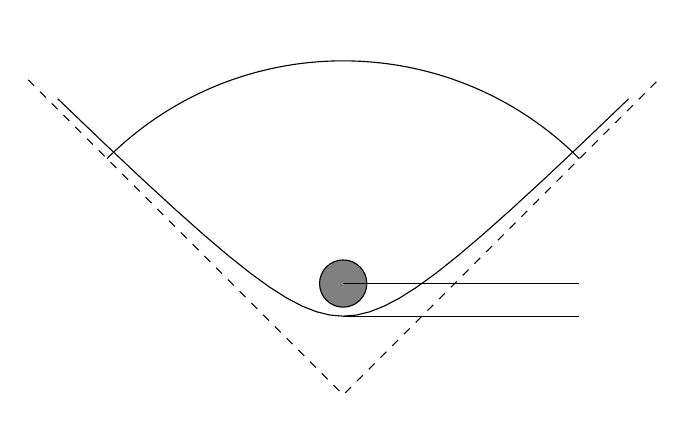
\begin{tikzpicture}
\draw[fill=gray] (0,{sqrt(2)}) circle (.3);
\draw [dashed] (-4,4)--(0,0)--(4,4);
\draw plot[domain=-2:2, thick] ({sinh(\x)},{cosh(\x)});
\draw (0,{sqrt(2)})--(3,{sqrt(2)});
\draw (0,1)--(3,1);
\draw[thin] (-3,3) arc (135:45:{3*sqrt(2)});
\end{tikzpicture}

진입속도 $v$, 근접거리 $r$.

\chapter{달 미션}

\part{매뉴버}
\part{미세조정 (Fine-tuning)}
\part{행성간 비행}
\chapter{시간계획 정하기}
\chapter{포획 (Capturing)}
행성계 외부에서 진입하는 물체는 탈출속도를 넘어서므로\footnote{정확히는 `행성계 관점에서 보았을 때 양(陽)의 에너지를 갖으므로'라고 하는 것이 옳을 것이다. `탈출속도'라는 개념은 보통 원궤도를 그리던 물체에 얼마만큼의 $\Delta v$가 주어져야 탈출할 수 있는지에 대한 얘기이다.} 힘이 작용하지 않으면 쌍곡선 궤도를 그리며 다시 행성계 밖으로 탈출하게 될 것이다.
안정적인 미션 수행을 위해서 행성간 미션에서는 도착지에서 충분히 감속하여 구속궤도를 만들 수 있는 기술이 필요하다. 이를 `포획'이라고 부르도록 하겠다. 포획이 이루어지지 않는다면 행성의 인공위성 궤도에 진입하는 미션을 수행할 수 없으며, 착륙 미션에 경우 한번만에 성공해야 하는 부담을 안게 된다.\footnote{비구속궤도(쌍곡선궤도)로부터 대기권으로 진입할 때, 높은 진입속력으로 인해 높은 열이 발생하게 되어 우주선이 소실될 위험성이 커지게 되며, 또한 다시 튕겨나가지 않고 충분히 감속할 수 있는 가능성도 줄어들게 된다.}

엔진을 이용한 능동적인 감속은 설명이 필요없으므로 여기서는 동력을 사용하지 않고 포획당하는 방법에 대해서 설명하고자 한다. 두가지 방법을 생각할 수 있을텐데, 행성의 대기를 이용한 방법과 행성의 위성을 이용한 방법이 있을 것이다. 각각의 방법에 대해서 설명하고자 한다.
\section{대기를 이용한 포획 (Atmospheric Capture)}
\section{위성을 이용한 포획 (Sling-shot Capture)}
다음은 위성을 이용한 슬링샷으로 행성계에서의 속도를 줄일 수 있는지 검토해 보도록 하자. 위성과 조우시 위성의 속도가 우주선의 반대방향이라면 위성의 운동량을 받아 감속할 수 있으리라고 예상할 수 있을 것이다. 하지만 행성간 여행에서 그렇게 정확한 타이밍을 맞출 수 있으리라고 기대하기는 어렵다. 이번 section에서는 행성계 진입후 주어진 상황에서 감속할 수 있는지에 대해 알아볼 것이다. 다음 section에서는 진입 타이밍을 조정하는 법에 대해 논의해 보겠다.

우선 행성과 위성은 충분히 멀리 떨어져 있어서 조우(encounter)를 탄성충돌로 근사할 수 있다고 가정할 것이다. 사실 KSP는 각 천체의 '영향권'내에서 1체문제로 환원함으로서 이러한 가정을 충실히 따르고 있다.
\section{포획을 위한 궤도조정 (Fine-tuning with Sling-shot Capture)}

\chapter{사례들}
\section{Juno's Maneuver}
\begin{enumerate}
\item 지구계를 탈출한다.
\item 약 2배의 공전궤도를 만들어 다시 지구와 만날 수 있게 한다.
\item 원일점에서 근일점을 낮게 하는 매뉴버를 실시하여 다음 매뉴버에서의 에너지 효율을 높인다.
\item 지구를 이용한 슬링샷 효과를 포함하여 목성과의 접점을 만든다.
\item 목성근체에서 목성과 비슷한 속도로 가속하여 목성궤도로 들어간다.
\end{enumerate}
\part{그 외 다루어지지 않은 것들}
\chapter{Aviation}
이번 chapter에서는 비행기로 비행시에 유용하게 쓸 수 있는 도표를 소개하고자 한다.

비행기의 비행속도 측정시에 IAS(Indicated Airspeed)라는 단위를 쓰게 된다. 
이는 비행기 바깥에 붙어있는 압력계를 이용하여 공기밀도를 표준밀도로 가정하고 공기의 유속을 추정한 결과로서, 베르누이 법칙($\rho v^2 + P = const$)을 고려해보자면 계기에 의해 측정되는 수치는 같은 유속일때 유체의 밀도의 (-1/2)승에 비레하게 될 것이다. (반대로 True Airspeed를 구하기 위해서는 측정된 압력차에 공기밀도의 제곱근을 곱하면 될 것이다.)

한편, 공기저항 또는 양력(lift)은 보통 저속에서 면적과 공기밀도에 비례하고 속도의 제곱에 비례한다는 공식을 쓴다. ($\sim \rho v^2 A$)
두 공식이 $\rho v^2$에 비례한다는 점에서 같으므로 양력은 IAS에만 의존하게 된다고 할 수 있다. (물론 고속에서 양력 공식이 변한다면 이 또한 달라질 것이다.)

저자가 실제로 게임 상에서 실험해본 바로는, 실제 지구처럼 시각에 따라, 태양복사에 따라 대기의 온도가 변하는 듯하지만, 위키에 제시된 Kerbin 표준 기온 도표에 따라 계산하도록 하겠다. \footnote{\url{http://wiki.kerbalspaceprogram.com/wiki/Kerbin}}

\paragraph{종단속도}
흡기하는 제트엔진의 추력은 어림잡아 공기밀도에 비례한다고 예상할 수 있다. (실제 게임에서는 어떤 모델을 쓰는지 모르겠음. 추가바람. 특히, 램제트 같은 고속에 특화된 엔진 및 흡기구의 경우 많이 달라질 수 있음.) 또한, 공기저항도 어림잡아 공기밀도에 비례하므로, 비행기의 종단속도는 고도에 따라 변하지 않는다고 예상할 수 있다.
\begin{figure}
\includegraphics[width=\textwidth]{ias.pdf}
\caption{test 참고로 대략적으로 IAS 60\,kt\,는 경비행기의 이착륙속도이고 IAS 160\,kt, 220\,kt는 각각 B747과 Concorde의 이착륙속도이다. IAS 370\,kt와 430\,kt는 747과 Concorde의 순항속도이다. 실제 지구에서 Concorde는 55,000\,ft에서 M\,2.0으로 항행하였다.}
\end{figure}

경험상 흡기엔진으로 구동하는 비행기가 항속 가능한 최대고도 및 속도는 23000\,m 및 1200m/s 정도였다. (정확한 자료 추가바람. 하지만 비행기의 모델에 따라 달라지므로 정말 '극한값'을 구할 수 있을지는 미지수.) 
또한, 흡기 자체는 26000\,m 까지 가능하였다. (속도에 따라 달라질 수 있다.)

\chapter{3체 문제 (Three Body Problem)}
\section{KSP의 간략화}
\section{근일점 변화}
\begin{align}
	\frac{d^2r^{-1}}{d\theta^2}+r^{-1}-GMl^{-2}-l^{-2}r^2V'(r) = 0
\end{align}
\begin{align}
	\frac{d^2r^{-1}}{d\theta^2}+r^{-1}-GMl^{-2}+2 l^{-2}r^3 \left(\frac{|\alpha_-| -|\alpha_+|}{2}+\frac{|\alpha_-| +|\alpha_+|}{2}\cos(\theta-\omega t)\right)= 0
\end{align}


\section{세차운동}
*로켓발사로 인한 변화
\\*애초에 축은 0도로 고정
\chapter{상대론적 문제}
\section{특수상대론: 로렌츠변환}
\section{특수상대론: 적색/청색편이}
\section{일반상대론적 효과 및 천체모델의 근사성}

\part{데이터 및 프로토콜}
\chapter{게임 데이터}
이 챕터의 내용은 주로 게임 내부 데이터 및 물리법칙에 대한 것이며, 따라서 저작권은 게임제작사에 있으며, 인용하고 있는 제3자의 저작권은 없는 것으로 해석합니다. (독창성 결여)
데이터는 게임 플레이 중 직접 확인할 수 있는 부분이며, 상이한 점을 발견하면 갱신 부탁드립니다.

\section{행성 데이터}
\begin{tabular}{|l|l|}
\hline
이름&
\end{tabular}
\section{위성 데이터}
\section{엔진 데이터}

\chapter{}

\backmatter
\backpage

\end{document}
